\documentclass[a4paper,12pt]{article}

\usepackage[utf8]{inputenc}
\usepackage[T1]{fontenc}
\usepackage{graphicx}
\usepackage{geometry}
\usepackage{subcaption}
\usepackage{setspace}
\usepackage{minted}
\usepackage{authblk}
\usepackage{caption}
\captionsetup[listing]{labelformat=empty}
\usepackage{amsmath}
\usepackage{amssymb}
\usepackage{regexpatch}
\usepackage{dsfont} 
\usepackage{mathrsfs}
\usepackage{array}
\usepackage{hyperref}
\usepackage{tikz}
\usetikzlibrary{trees}
\usetikzlibrary{positioning}
\usepackage{xcolor}
\usepackage{pgfkeys}
\usepackage{booktabs}
\usepackage{listings}
\usepackage[linesnumbered,ruled,vlined]{algorithm2e}
\usepackage[noend]{algpseudocode}
\usepackage{fancyhdr}
\setlength{\parindent}{0pt}
\geometry{a4paper, margin=2.5cm}

\sloppy
\begin{document}

\begin{titlepage}

    \vspace*{4cm}

    \centering
    
    
\includegraphics[width=0.6\textwidth]{Images/logo.png} \\[1.5cm]
    
    \rule{\linewidth}{1pt} \\[1cm]

    {\Huge \bfseries HAX907X - Apprentissage statistique}\\[0.5cm]
    {\Huge TP : Support Vector Machines (SVM)}\\[1cm]
    
    \rule{\linewidth}{1pt} \\[2cm]

    {\Large \textbf{Marine GERMAIN}}\\
    {\Large \textbf{Coralie ROMANI DE VINCI}}\\[1cm]
    

\end{titlepage}


\renewcommand{\contentsname}{Table des matières}
\tableofcontents


\newpage

\section{Base de données Iris}

Dans cette section, nous étudierons la base de données Iris sur laquelle nous ferons une étude de classification sur les classes $1$ et $2$.
Nous utiliserons d'abord le noyau linéaire puis le noyau polynomial et nous les comparerons.
Nous avons séparé le dataset en deux parties : un ensemble d'entraînement (75\% des données) et un ensemble de test(25\% des données). 

\subsection{Classification avec noyau linéaire}

La classification des deux premières variables avec un noyau linéaire à pour objectif de trouver une hyperplan qui sépare au mieux les deux classes en maximisant la marge entre les points les plus proches de chaque classe. 
Les scores obtenues pour cette méthode sont les suivants :

\begin{figure}[h!]
    \centering
    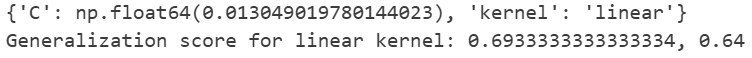
\includegraphics[width=0.8\textwidth]{Images/linear_score.png}
    \caption{}
    \label{fig:linear}
\end{figure}

Pour les données d'entraînement, le modèle a classifié correctement 69,3\% des données, contre 64\% pour les données de test. 


\subsection{Classification avec noyau polynomial}

La classification des deux premières variables avec un noyau polynomial à pour objectif de trouver une frontière de décision non linéaire capable de séparer au mieux les deux classes. 
Nous souhaitons ici voir si l'emploi d'un noyau polynomial nous permet d'obtenir un meilleur classifieur que celui obtenu précédemment.\\
Les scores obtenues pour cette méthode sont les suivants :

\begin{figure}[h!]
    \centering
    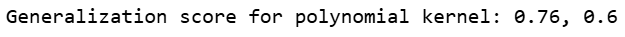
\includegraphics[width=\textwidth]{Images/poly_score.png}
    \caption{}
    \label{fig:poly}
\end{figure}

Pour les données d'entraînement et de test, le modèle a classifié correctement 68\% des données. \\

\textbf{Comparaison des deux méthodes :}\\[0.5cm]
- Nous disposons d'abord des scores obtenus en figure \ref{fig:linear} et figure \ref{fig:poly}.
On remarque que le score pour le noyau linéaire est très légèrement plus élevé que celui du noyau polynomial pour les données d'entraînements $0.693$ contre $0.68$.
En revanche il est légèrement plus faible pour les données de test $0.64$ contre $0.68$. A noter que ces différences sont faibles et que ces deux méthodes semblent donc similaires.\\

- Ensuite, nous avons tracé graphiquement ces résultats à l'aide des frontières : \\
\begin{figure}[h!]
    \centering
    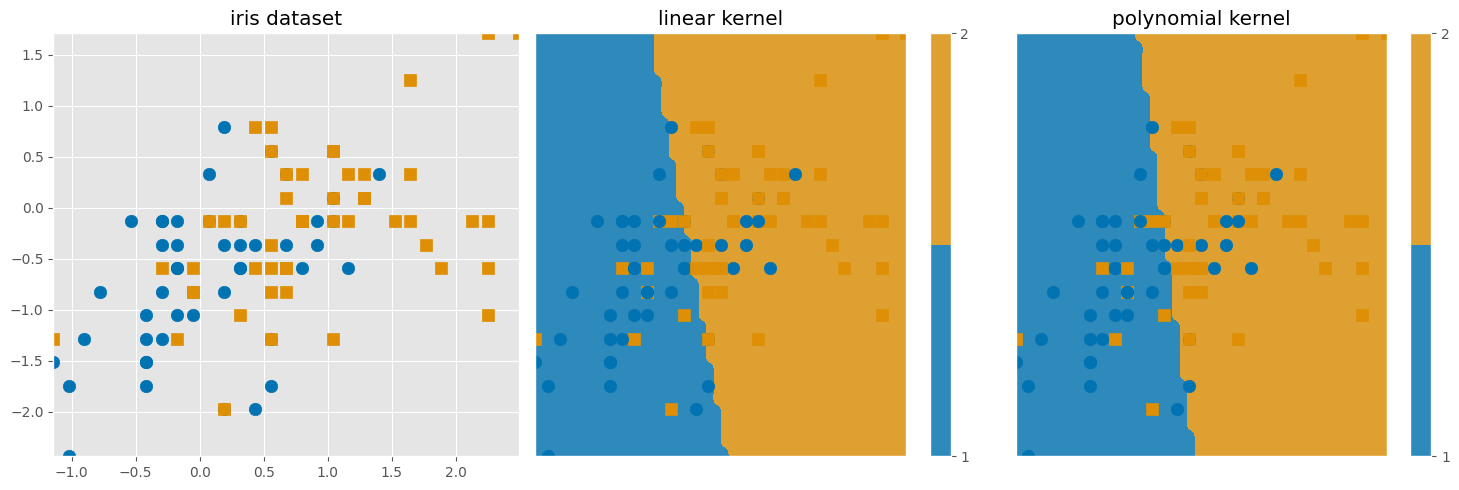
\includegraphics[width=0.8\textwidth]{Images/linear_vs_poly.png}
    \caption{}
    \label{fig:compare}
\end{figure}

La figure \ref{fig:compare} permet de visualiser les deux classifieurs sur l'ensemble des données du dataset Iris.\\
On observe que la frontière du noyau polynomial semble plutôt linéaire.
La différence remarquable est que pour le noyau linéaire on observe qu'il y a moins de données "bleues" mal classifiées que pour le noyau polynomial.
On peut faire l'observation inverse concernant les données "oranges".
A REFORMULER + CONCLURE 

\section{SVM GUI}

Nous utilisons dans cette section le script \texttt{svm\_gui.py}.\\

\section{Classification des visages}

\subsection{Influence du paramètre de régularisation}

\subsection{Variable de nuisances}

\subsection{Réduction de dimensions}

\end{document}